\section{Quantenhardware}
\label{sec:quantenhardware}

Die Realisierung eines Quantencomputers ist durch hohe technische herausforderungen geprägt. Um die besonderen Eigenschaften der Qubits eines Quantencomputers, wie Superposition und Verschränkung, zu nutzen können müssen sie durch externe Einflüsse geschützt werden und die Dekoheränz minimiert werden.

Aüßere Einflüsse wie Temperaturschwankungen, elektromagnetische Felder oder Strahlung aller art können die Qubits beeinflussen. Aus diesem Grund werden Quantencomputer bei extrem niedrigen Temperaturen und in einem Vakuum betrieben.

\subsection{Dekohärenz}
\label{sub:dekohaerenz}
Dekoheränz ist ein zentrales Konzept welches wichtig in der Entwicklung von Quantencomputern ist. Der Prozess der Dekoheränz beschreibt den verlust der koheränten Quanteneigentschaften eines Qubits durch Wechselwirkung mit der Umgebung.
Diese Veränderung führt zu einem Übergang von quantenmechanischem Verhalten zu einem klassischem.\\

In der Quantenmechanik können Systeme in Überlagerungszuständen existieren, wobei mehrere Zustände gleichzeitig eingenommen werden können. Diese Eigenschaft erklärt auch das Phänomen der Quanteninterferenz.
Äußeren einflüsse durch die Umgebung kann eine Verschränkung der beiden, diese Verschränkung führt dazu, dass die Phasenbeziehungen zwischen den Komponenten der Überlagerung zerstört werden.
Folgernd verliert das System die Interferenzeffekte und verhält sich zunehmend klassischer, diese Zeit nennt man Dekoheränzzeit.\\

Die \textbf{Dekoheränzzeit} ($T_2$) eines Qubits misst die läge der Zeit in der er in der lage bleibt kohärent zu bleiben, welcher danach von äußeren Einflüssen zerstört wird.
Neben $T_2$ wird auch häufig die \textbf{Relaxationszeit} ($T_1$) gemessen, welche angibt, wie lange ein Qbit im angeregten Zustand bleibt, bevor er auf sein Grundzustand zurückfällt.
In der Realität ist die Dekoheränzzeit jedoch in den meisten fällen kürzer als die Relaxationszeit.\\

\textbf{Berechnung der Dekoheränzzeit}\\
Durch eine Messung der zeitlichen abnahme der Koheränz eines beispielhaften Qubits kann die Dekoheränzzeit eines Systems festgelegt werden.
Bei einem Quantencomputer der auf dem Spin eines Teilchen beruht kann dies durch die \textbf{Spin-Echo-Methode} gemacht werden.
Quantencomputer die auf anderen Quantenbits basieren haben equivalente Methoden um die Kohärenz zu messen.\\

Das einfachste Modell zur Beschreibung der Dekoheränzzeit ist die \textbf{Exponentielle Abnahme der Kohärenz}

\begin{equation}
    C(t) = C(0)*e^{-t/T_2}
\end{equation}

Dabei ist:\\
$C(t)$ Die Kohärenz des Qubits zum Zeitpunkt t\\
$C(0)$ Die initiale Koheränz\\
$T_2$ Die Dekoheränzzeit\\

Indem man den Kohärenzverlust experimentell misst und die Werte in eine exponentielle Abklingfunktion einpasst, erhält man $T_2$\\

\begin{tcolorbox}[title=Kommentar,
    title filled=false,
    colback=cyan!5!white,
    colframe=cyan!75!black]
    Die \textbf{Dekoheränzzeit} kann auch durch genauere jedoch auch deutlich kompliziertere weise errechnet werden.
    Bekannte Methoden hierfür wären zum Beispiel die Spektrale Analyse, Dynamische Entkopplung, Hahn-Echo und Ramsey-Interferometrie.
    Außerdem wird duch das häufige messen der Dekoheränzzeit diese indirekt verlänger. Diesen Effekt nennt man Quanten-Zeno-Effekt.\\
    Zuletzt muss auch die Lindblad-Gleichung genannt werden welche den Zeitverlauf der Dichtematrix in einem Offenen Quantensystem beschreibt.
    \begin{equation}
        \frac{dp}{dt} = -i[H,p]+\sum_i(L_ipL^\dagger_i-\frac{1}{2}\{L^\dagger_i L_i,p\})
    \end{equation}
    Diese Themen sprengen jedoch den Rahmen dieser Arbeit in Richtung Physik und werden deswegen nicht weiter behandelt.
\end{tcolorbox}

\subsection{Universelle Quantencomputer}
\label{sub:universelle_quantencomputer}
Universelle Quantencomputer beruhen grundlegend auf einem Gate Modell wie bereits in diesem Artikel beschrieben. Folgend sind drei der meist erforschten
Methoden dieses Modell Physikalisch umzusetzen.

\subsubsection{Superleitenden Qubits}
\label{subsub:superleiter}
Quantencomputer mit Supraleitern funktionieren mit elektrischen Schaltkreisen, die bei temperaturen nahe dem absoluten Nullpunkt betrieben werden. Solche temperaturen sind nötig
um die supraleitende Eigenschaft aufrecht zu erhalten.\\

Zwei häufig benutze Qubit-Typen dieser elektrischen Schaltkreisen sind:\\
\textbf{Transmon-Qubits}, basiert auf der Ladung des Energieniveaus welche durch eine Josephson-Junktion kontrolliert wird.\\
\textbf{Flux-Qubits} werden auch durch Josephson-Junktions kontrolliert, beruhen jedoch auf dem magnetischen Fluss in der Schleife.\\

Beide Ansätze basieren auf dem \textbf{Josephson-Effekt}, welcher auftritt wenn ein supraleitender Strom durch eine dünne Isolierschicht zwischen zwei Supraleitern fließt.\\
Dieser Effekt hat zur folge das eine nichtlineare Spannung-Stom-Beziehung erntsteht und für die Manipulation von Qubits genutzt wird.\\

\begin{figure}[!ht]
    \centering
    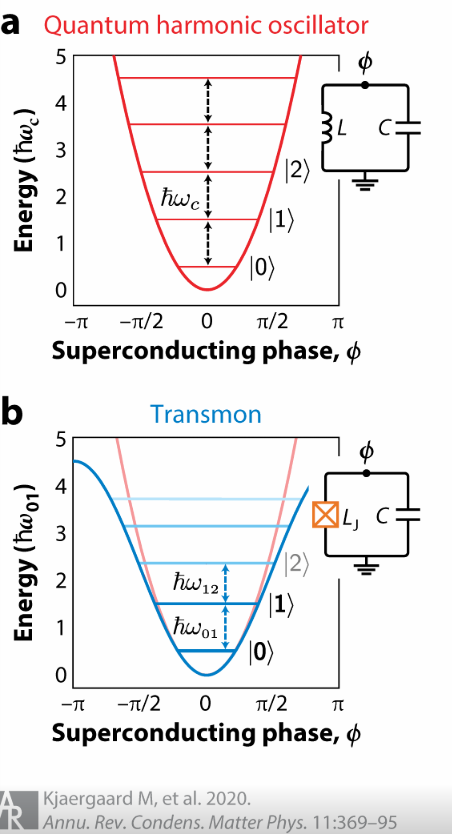
\includegraphics[width=0.75\linewidth]{img/JJ.png}
    \caption{Josephson-Effekt mit einem Josephson Junktion}
    \label{fig:Josephson-junktion}
\end{figure}

In der vorliegenden Abbildung wird der unterschied zwischen einer harmonischen Quantenschwankung (a) und der nicht Lineare Schwankung des Energieniveau der Josephson Junktion (b) abgebildet.\\

Der Phasenunterschied bei der harmonischen oscellation, gekennzeichnet als $\hbar\omega_c$, ist identisch. Auf der Abbildung ist zu sehen das das Energieniveau der Phasen zwischen $\ket{0} \leftrightarrow \ket{1}$
und $\ket{1} \leftrightarrow \ket{2}$ identisch ist, und dadurch nicht unterschieden werden kann zwischen welche Phase gewechselt wurde.\\

Mit einer Josephson Junktion kann jedoch eine nichtlineare Schwankung des Energieniveaus erreicht werden, welche auf der Abbildung als orangenes  gekennzeichnet ist (b).
Durch diese nichtlineare Schwankung ist das Energieniveau zwischen den Phasen $\ket{0} \leftrightarrow \ket{1}$ und $\ket{1} \leftrightarrow \ket{2}$ unterschiedlich und kann somit unterschieden werden.
Der als $\hbar\omega_{01}$ gekennzeichnete Energieunterschied ist unser Qubit\\

\textbf{Steuerung und Auslesung}\\
Die Steuerung der Josephson-Junktion erfolgt durch Mikrowellenpulse, welche die Energie des Qubits verändern. Die Auslesung erfolgt durch eine Mikrowellenresonanz, welche die Energie des Qubits misst.\\

\subsubsection{Topologische Quantencomputer}
\label{subsub:topologische_quantencomputer}
Die Funktionsweise von Topologische Quantencomputer unterscheidet sich hauptsächlich auf welche Art sie Quantenbits erzeugen.
Im gegensatz zu den vorher genannten Ansätzen, welche ihre Quantenbits auf Eigenschaften von einzelne Protonen oder Elektornen basieren, sind Quantenbits in Topologischen Quantencomputern aus einer größeren Anzahl von Elektornen aufgebaut.
Diese zusammengesetzten Elektronen werden als Majorana Partikel bezeichnet und treten nur in paaren auf. Durch die Verwendung von Majorana Partikeln wird die Dekohärenz der Quantenbits minimiert, da Majorana Partikel durch ihre topologischen Eigenschaften gegenüber Störungen weniger empfindlich sind.
Vorstellen kann man sich dies wie eine Brücke welche dürch die Majorana Partikel gebildet werden auf welcher sie die Elektornen bewegen. Diese Brücke wird durch eine 
Es bleibt jedoch die frage wie mit diesen Majorana Partikeln Quantenbits erzeugt werden können. Wie vorher beschrieben basieren Topologische Quantencomputer nicht auf einem einzelnen Elektorn sondern 

\subsubsection{Quantenpunkte}
\label{subsub:quantenpunkte}
Quantencomputer basierend auf Quantenpunkten auch Quantum-Dot genannt nutzen winzige Halbleiterstrukturen um Qubits zu realisieren.
Quantum-Dots sind künstlich erzeugte Nano-Partikel, in denen Elektronen in drei Dimensionen eingeschlossen sind, was zu quantisierten Einergiezuständen führt.\\

Die größe eines Quantum-Dots typischerweise 2-10 Nanometer, und es schließt eine kleine Anzahl oder ein einzelnes Elektron ein.
Für die fertigung werden oftmals Galliumarsenid (GaAs) oder Silizium (Si) verwendet. Der physikalische einschluss der Elektronen schränkt ihre
Bewegung stark ein, wodurch ein quantisiertes Energienivea entsteht. Dies ähnelt den Energieniveaus eines Atoms, weswegen Quantum-Dots auch als künstliche Atome bezeichnet werden.\\

